\documentclass[a4paper,14pt]{extarticle}
\usepackage{../../tex-shared/preamble}

\renewcommand{\mylabnumber}{1}
\renewcommand{\mylabtitle}{Исследования способов построения и
                           особенностей функционирования
                           аналого-цифровых преобразователей}
\renewcommand{\mysubject}{Технические средства информационных систем}
\renewcommand{\mylecturer}{Дрозин А.Ю.}

\begin{document}
\begin{titlepage}
    
    \thispagestyle{empty}
    
    \begin{center}
        
        Министерство науки и Высшего образования Российской Федерации \\
        Севастопольский государственный университет \\
        Кафедра ИС
        
        \vfill

        Отчет \\
        по лабораторной работе №\mylabnumber \\
        \enquote{\mylabtitle} \\
        по дисциплине \\
        \enquote{\MakeTextUppercase{\mysubject}}

    \end{center}

    \vspace{1cm}

    \noindent\hspace{7.5cm} Выполнил студент группы ИС/б-17-2-о \\
    \null\hspace{7.5cm} Горбенко К. Н. \\
    \null\hspace{7.5cm} Проверил \\
    \null\hspace{7.5cm} \mylecturer

    \vfill

    \begin{center}
        Севастополь \\
        \the\year{}
    \end{center}

\end{titlepage}
\section{Цель работы}
Изучение принципов преобразования аналоговых процессов в цифровые
и особенностей схемной реализации аналого-цифровых преобразователей
(АЦП), исследование зависимостей, приобретение практических
навыков моделирования АЦП и измерения параметров сигналов в
характерных точках АЦП.

\section{Ход работы}
\subsection{Схема АЦП}
Структурная схема аналого-цифрового преобразователя изображена
на рисунке \ref{fig:scheme}.
\begin{figure}[H]
    \centering
    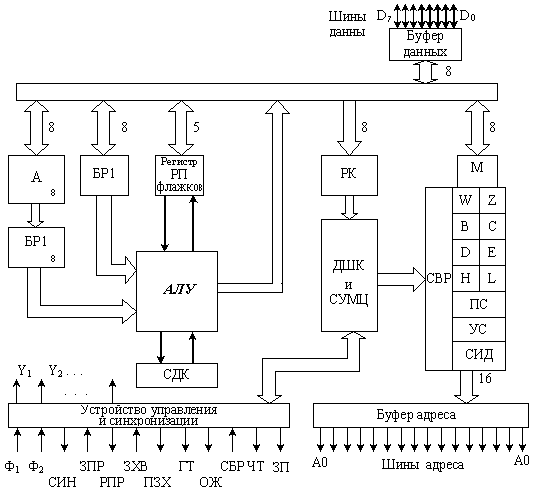
\includegraphics[width=\linewidth]{scheme}
    \caption{Схема аналого-цифрового преобразователя}
    \label{fig:scheme}
\end{figure}

Шаг квантования АЦП:
\begin{equation}
    h = \frac{U_{max}}{2^N - 1} = \frac{5}{256 - 1} = 0.02 \; B. 
\end{equation}

\subsection{Результаты измерений}
На рисунках представлены результаты измерения зависимости выходного
кода от входного напряжения.
\begin{enumerate}
    \item $U = 0 \; B., N = 00000001_{2}$.
        \begin{figure}[H]
            \centering
            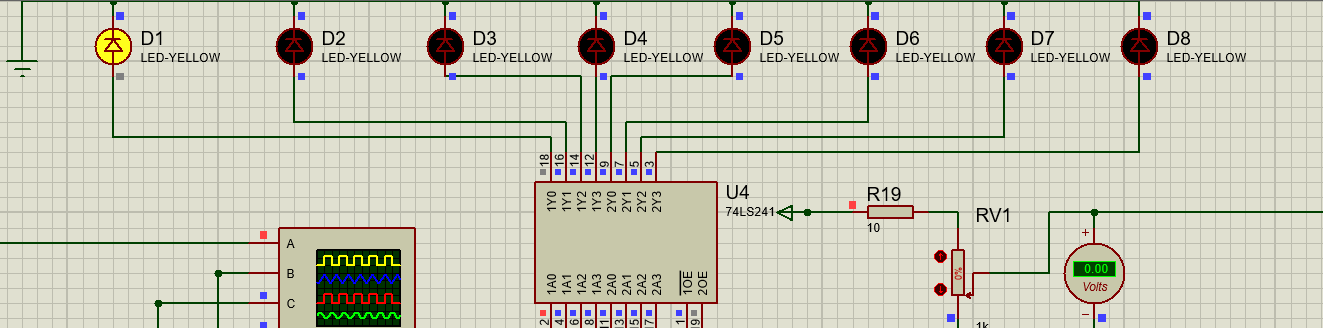
\includegraphics[width=\linewidth]{0v}
            \caption{Выходной код при U = 0 В.}
            \label{fig:0v}
        \end{figure}
    \item $U = 1 \; B., N = 00110011_{2}$.
        \begin{figure}[H]
            \centering
            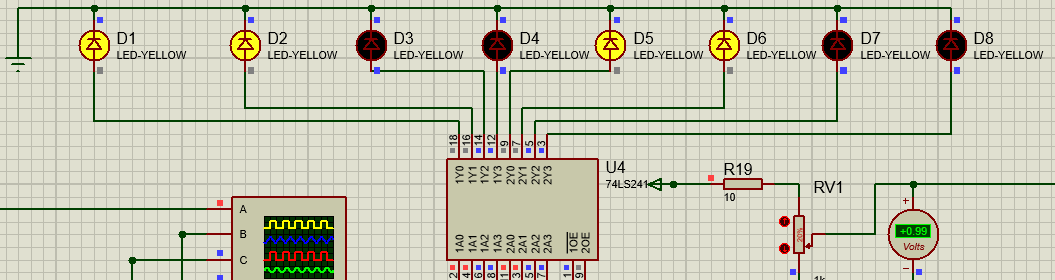
\includegraphics[width=\linewidth]{1v}
            \caption{Выходной код при U = 1 В.}
            \label{fig:1v}
        \end{figure}
    \item $U = 2 \; B., N = 01100110_{2}$.
        \begin{figure}[H]
            \centering
            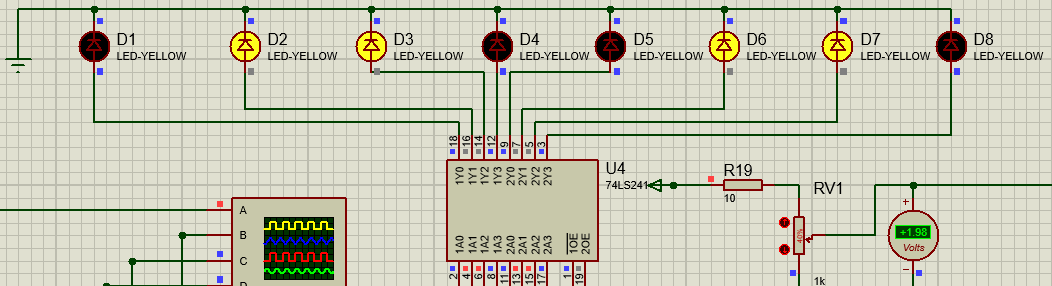
\includegraphics[width=\linewidth]{2v}
            \caption{Выходной код при U = 2 В.}
            \label{fig:2v}
        \end{figure}
        \pagebreak
    \item $U = 3 \; B., N = 10011001_{2}$.
        \begin{figure}[H]
            \centering
            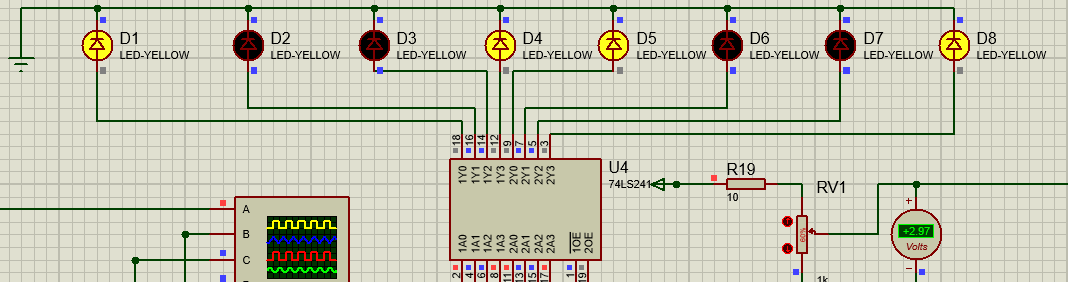
\includegraphics[width=\linewidth]{3v}
            \caption{Выходной код при U = 3 В.}
            \label{fig:3v}
        \end{figure}
    \item $U = 4 \; B., N = 11001111_{2}$.
        \begin{figure}[H]
            \centering
            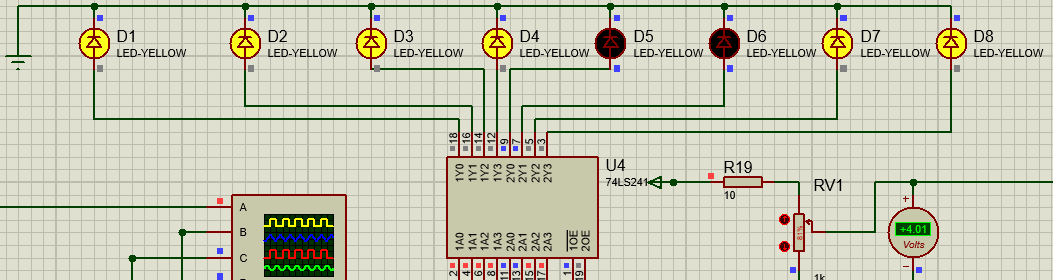
\includegraphics[width=\linewidth]{4v}
            \caption{Выходной код при U = 4 В.}
            \label{fig:4v}
        \end{figure}
    \item $U = 5 \; B., N = 11111111_{2}$.
        \begin{figure}[H]
            \centering
            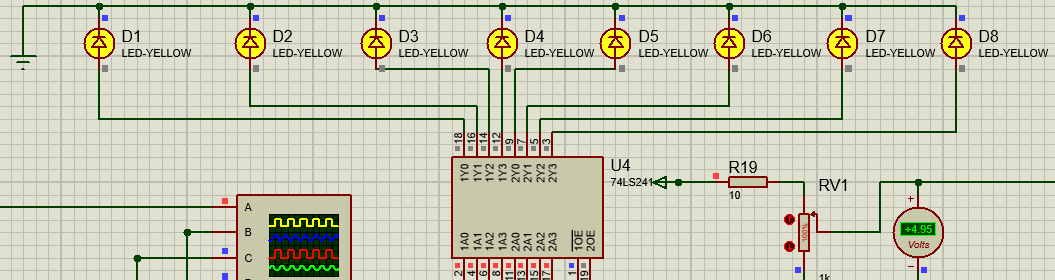
\includegraphics[width=\linewidth]{5v}
            \caption{Выходной код при U = 5 В.}
            \label{fig:5v}
        \end{figure}
\end{enumerate}
\section*{Выводы}
В ходе лабораторной работы были изучены принципы преобразования аналоговых
сигналов в цифровые и особенности схемной реализации АЦП последовательного
счета. В результате работы была реализована схема 8-битного АЦП.

У полученного АЦП минимальное значение напряжения больше шага квантования,
следовательно, на выходе не может установиться нулевой код.
\end{document}